\documentclass[10pt, a4paper]{article}
\usepackage[margin=1in]{geometry}
\usepackage{cmbright}
\usepackage[OT1]{fontenc}
\usepackage{authblk}
\usepackage{siunitx}
\usepackage[british]{babel}
\usepackage{csquotes}
\usepackage[backend=biber, style=numeric]{biblatex}
\usepackage{multicol}
\usepackage{amsmath}
\usepackage{enumitem}
\usepackage{booktabs}
\usepackage[hidelinks]{hyperref}
\usepackage{tabularx}
\usepackage[labelfont=bf, textfont=normalfont, justification=raggedright, singlelinecheck=false, font=small]{caption}
\usepackage{float}
\usepackage{titlesec}
\titleformat{\section}
  {\normalfont\bfseries}
  {\thesection}{1em}{}
\titlespacing*{\section}{0pt}{1.2\baselineskip}{0.6\baselineskip}
\titleformat{\subsection}
  {\normalfont\itshape}
  {\thesubsection}{1em}{}
\titlespacing*{\subsection}{0pt}{1\baselineskip}{0.4\baselineskip}
\DeclareSIUnit\mmHg{mmHg}
\DeclareSIUnit\bar{bar}
\usepackage{graphicx}
\usepackage{fancyhdr}
\addbibresource{references.bib}

\newcommand{\pulsepumpdocbase}{https://pulsepump.github.io/pulsepump/api/core.html}
\newcommand{\Programme}{\underline{\href{\pulsepumpdocbase\#pulsepump.core.programme.Programme}{\texttt{Programme}}}}
\newcommand{\Block}{\underline{\href{\pulsepumpdocbase\#pulsepump.core.programme.Block}{\texttt{Block}}}}
\newcommand{\FunctionGenerator}{\underline{\href{\pulsepumpdocbase\#pulsepump.core.programme.FunctionGeneratorSource}{\texttt{FunctionGenerator}}}}
\newcommand{\OpenBF}{\underline{\href{\pulsepumpdocbase\#pulsepump.core.programme.OpenBFSource}{\texttt{OpenBF}}}}

\title{
    Interim Individual Report\\[0.5em]
    \Large Team 2: Low Cost Perfusion Pump, \textit{PulsePump}\\[0.25em]
    \normalsize Part IIA: \texttt{GM1} \textit{Multidisciplinary Design}
}

\author[1]{Tahmid Azam\footnote{In the work carried out, Claude has been used to help brainstorm and research ideas. It has also been used to check the content against the assessment criteria.
Claude Code has been used to write code according to defined software requirements (e.g. generating a UI according to a strict design brief); refactor classes and help identify different strategies for abstractions.
In this report, all prose writing is original.
Claude Code has been used to help debug \LaTeX errors, correct formatting syntax, and help adhere to best \LaTeX practices.
I am happy to share Claude Code transcripts in person if required (exporting them is proving difficult).
The use of LLMs has been engineered using developer tooling (language servers, linting, formatting, typechecking, documentation) alongside specific prompting techniques and skills (user grilling using questions, Git subtrees of specific python libraries to provide access to module source code) to reduce hallucinations, improve code quality, and achieve greater progress than conventional coding in 10 days.}}
\affil[ ]{{\normalsize with teammates Luca Buxton, India Henry, Lonnie McKiernan, and Lucy Payne}}
\affil[ ]{{\normalsize mentored by Dr. Peter Long and Prof. Athina E. Markaki}}
\affil[ ]{{\small}}
\affil[1]{Department of Engineering, University of Cambridge}

\date{Sun 24 May 2026}

\begin{document}
\maketitle

\pagestyle{fancy}
\fancyhf{}
\fancyhead[L]{\small Team 2: Low cost perfusion pump, \textit{PulsePump} \textit{}}
\fancyhead[R]{\small Interim Individual Report}
\fancyfoot[C]{\thepage}
\thispagestyle{plain}

\paragraph{External resources}
\begin{itemize}
  \item You can find the repository for this report (\LaTeX source) here: \underline{\href{https://github.com/tahmidazam/gm1-interim}{tahmidazam/gm1-interim}}
  \item You can find the repository for the project here: \underline{\href{https://github.com/PulsePump/pulsepump}{pulsepump/pulsepump}}.
  \item You can find the documentation website here: \underline{\href{https://pulsepump.github.io/pulsepump/}{pulsepump.github.io}}. A development log can be found here: \underline{\href{https://pulsepump.github.io/pulsepump/devlog/index.html}{pulsepump.github.io/devlog}}.
\end{itemize}

\newpage

\section{Work completed}

\subsection{Requirements and use case analysis (1 hour)}

We chose a waterfall software development model with the capacity for more interative development during integration with control.
The software requirements were developed further from the short team report, due to recognising the need to have effective sofware designed for use by the rest of the team to connect and test peripherals (stepper motors, servos, pressure sensors), and view and debug signals.
Two use cases emerged, for which solution-neutral problem statements involve:

\begin{enumerate}[noitemsep]
  \item a means to configure a collection of actuators and sensors, observe their behaviour as it happens, and preserve a record of it for later review; and
  \item a means to specify a target pressure waveform for an artificial pump, expressed in a compact, human-readable form that can be shared between researchers and reproduced from published descriptions.
\end{enumerate}

We better understood the lifecycle of the processes associated with running a session, a user story:

\begin{enumerate}[noitemsep]
  \item The researcher configures a particular target pressure waveform for a session of specified duration (e.g. \SI{90}{\min}).
  \item The researcher connects the Raspberry Pico via USB, sends this to the Raspberry Pico, and begins the trial, with the ability to monitor the session live (viewing live plots of the target and actual pressure).
  \item The researcher unplugs the Raspberry Pico from their device.
  \item The researcher may return during the session, plugging in the Raspberry Pico, in order to check how the session is going.
  \item The researcher may return long after the session has finished, and can download the full logs of all signals collected by the Pico during the run.
  \item The researcher can provide details on the configuration of the pump in their literature as human-readable, serialised files.
\end{enumerate}

We better understood the user stories behind members of the team running tests of peripheral devices connected to the Pico:

\begin{enumerate}[noitemsep]
  \item The engineer connects the Raspberry Pico their device and can verify that the firmware has been flashed and a bidirectional communication channel is opened.
  \item The engineer connects peripheral devices (e.g. pressure sensors, stepper motors, servos) to the Raspberry Pico.
  \item The engineer configures these devices (e.g. datasheet constants, pin assignment) in the software, and is warned if incompatible pins are selected (e.g. UART-capable, ADC-capable).
  \item The engineer can view all data readouts from their peripheral devices, and can configure live plots in the user interface to visualise these signals.
  \item The engineer starts a recording session, carries out tests, and ends it, saving all information related to the run in a folder on disk for later reference.
\end{enumerate}

\subsection{Programme Data Model (3 hours)}

We defined a \Programme{} representing a complete description of a target pressure profile for a duration of time, composed of \Block{}s, which can be defined and generated by a source.
Each \Block{} specifies the number of cycles for which it is repeated.
Sources currently include: a \FunctionGenerator{}, which supports sinusoidal, pulse, square, triangular, constant, and sawtooth waves; and \OpenBF{}, an open-source blood flow simulator \cite{openBF.jl-2018, wreo19175}.
The \Programme{} also defines the pressure unit and the sample rates.
This implementation uses run-length encoding (RLE) to dramatically reduce the file sizes required to be transferred over to the Raspberry Pico: instead of storing an array of all of the samples for the whole duration, we define a block and how many times it repeats, storing only one cycle's samples as a base-64 \texttt{float32} byte string.
The \Programme{} is serialised to the YAML file format so definitions of each \Block{} can be read by humans without the user interface.

Rather than implement the modelling pipeline from scratch, we have since opted to integrate openBF \cite{openBF.jl-2018, wreo19175}, an open-source 1D Navier-Stokes blood flow solver, allowing the solo development effort to be redirected toward software requirements analysis, user interface design, and the ergonomics of the tool.
The motivation for this change of heart was the time constraints surrounding the project.
The abstraction of Blocks being driven by a source with a set of configurable parameters also allows individuals to extend the functionality of the project by adding new sources (e.g. other blood flow simulation tools).

\subsection{Design (10 hours)}

The design for the programme editor involves a 3-panel layout: a sidebar, a preview, and an inspector, shown in \autoref{fig:programme-editor}.
On the left is a sidebar listing all of the blocks in the file.
Clicking on a block moves the preview panel's focus to one cycle of the selected block.
The preview renders the target pressure profile for the duration of the session, the keyboard shortcut \texttt{Mod+0} rescales to fit the whole session in the preview.
The inspector panel is where the \Programme{} and selected blocks are configured.
In the menu bar, standard file operations are included: \texttt{New}, \textit{Open}, \textit{Save...}, \textit{Save As...}; along with their standard operating system keyboard shortcuts.
You can switch the entire user interface to just view the source YAML file under the View Menu.

The design for the hardware bench involves a panel-based layout so each team member can easily customise the interface to better suit them, shown in \autoref{fig:hardware-bench}.
The panels include:

\begin{itemize}[noitemsep]
  \item A central signals panel (this is not removable), which lists each device and the signals it emits. For example, for a pressure sensor this is the raw counts of the ADC (a 16-bit binary value), along with this value transformed as a voltage, and a pressure according to the pressure sensor's datasheet.
  \item A connection panel which manages selecting the port to communicate to the Raspberry Pico on, and confirms successful connection.
  \item A run panel that allows for the starting and stopping of runs, and easy opening of the run folder in the operating system file explorer.
  \item A plot panel that allows for the dragging and dropping of signals from the signals panel for live plotting. Plotting panels can be added and removed such that there are more than 1 on the screen. They can be opened as separate windows too.
  \item A peripheral panel for each type of peripheral (e.g. stepper motor, pressure sensor, servo) that allows for the configuration of each peripheral (datasheet values, pin assignments).
\end{itemize}

For both applications, a bottom status bar that reports any errors and confirms updates to the Pico's internal state.

\subsection{Technology stack and tooling (2-3 hours)}

We chose a technology stack by evaluating against project requirements: first enumerating and weighting selection criteria (\autoref{tab:weights}), researching candidates (\autoref{tab:candidates}), and constructing a Pugh matrix (\autoref{tab:pugh}).
From the Pugh matrix, we chose Qt/PySide6/PyQtGraph.
It has a mature, panel-based layout engine, allowing for customisable and flexible docking of panels in various positions, and the opening of panels as separate windows as an extra benefit.

\subsection{Additional work (10-15 hours, collaborative)}

Alongside the work scoped to the software domain of the project, I have had the pleasure of collaborating with Lonnie and India on the electrical side, learning about microcontrollers, breadboards, jumper cables, use of function generators, power supplies, oscilliscopes, multimeters, stepper motors, servos, pressure sensors.
I have also conversed with Lucy and Luca on the mechanical side, attempting to explore their use of CAD and their design processes too.
I have also helped with various testing and construction of rigs.

\begin{table}[H]
  \small
  \centering
  \caption{Weighted selection criteria for GUI technology stack}
  \label{tab:weights}
  \begin{tabularx}{\textwidth}{XXc}
    \toprule
    criteria                         & description                                                                       & weight \\
    \midrule
    Cross-platform support           & Runs on Windows, macOS, and Linux                                                 & 5      \\
    Single codebase                  & Avoids fragmentation across platforms                                             & 5      \\
    UI framework maturity            & Breadth and stability of UI components                                            & 4      \\
    Scientific (plotting) capability & Quality and performance of visualisation tools and scientific computing functions & 5      \\
    Developer familiarity            & Existing team experience with stack                                               & 4      \\
    Python/MicroPython compatibility & Enables code reuse with Pico firmware (DRY principle)                             & 5      \\
    Development velocity             & Iteration speed, tooling, and DX                                                  & 4      \\
    Packaging/deployment             & Ease of distribution and environment management                                   & 3      \\
    \bottomrule
  \end{tabularx}
\end{table}

\begin{table}[H]
  \small
  \centering
  \caption{Candidate GUI technology stacks: strengths and weaknesses}
  \label{tab:candidates}
  \begin{tabularx}{\textwidth}{lXX}
    \toprule
    stack                 & strengths                                                                                                                  & weaknesses                                                                \\
    \midrule
    Qt/PySide6/PyQtGraph  & Mature desktop framework; excellent scientific ecosystem integration; high-performance real-time plotting; rapid iteration & Python packaging complexity; higher memory usage                          \\
    Electron/React/Plotly & Modern web ecosystem; fast UI development; strong cross-platform distribution                                              & High runtime overhead; weak scientific integration; no MicroPython parity \\
    Qt/C++                & Maximum performance; mature tooling; deep hardware integration                                                             & Slow iteration; high engineering complexity                               \\
    Avalonia UI/C\#       & Modern cross-platform .NET UX; good desktop tooling                                                                        & Smaller ecosystem; weaker scientific support                              \\
    GTK/Python            & Strong Linux integration; Python scientific ecosystem access                                                               & Less polished Windows/macOS UX                                            \\
    wxPython              & Lightweight; native look-and-feel                                                                                          & Smaller ecosystem; dated tooling                                          \\
    Web application only  & Highly portable; simple deployment; modern UI patterns                                                                     & Limited hardware access; offline limitations                              \\
    \bottomrule
  \end{tabularx}
\end{table}

\begin{table}[H]
  \small
  \centering
  \caption{Pugh matrix weighted scores by stack}
  \label{tab:pugh}
  \begin{tabularx}{\textwidth}{Xc}
    \toprule
    stack                 & weighted score \\
    \midrule
    Qt/PySide6/PyQtGraph  & 166            \\
    Web application only  & 143            \\
    Electron/React/Plotly & 135            \\
    GTK/Python            & 131            \\
    wxPython              & 130            \\
    Qt/C++                & 124            \\
    Avalonia/C\#          & 108            \\
    \bottomrule
  \end{tabularx}
\end{table}

Development tooling is critical for LLM-based agentic coding platforms to have feedback on linting (styling) errors, compilation errors (N.B., in intepreted Python this more concerns itself with type errors), and allows LLMs to rely on external tools for code formatting.
Running linting, formatting, and typechecking in continuous integration/continuous deployment pipelines prohibits the pushing of unsafe code that does not conform to best Python practices.
In addition, as development is collaborative and takes place on multiple machines across separate platforms, a unified Python toolchain is desired that handles syncing of Python virtual environments, dependencies, and prescribes opinionated ways for running the project.
We chose uv as the project orchestrator (handling project dependencies, defining and syncing Python environments), ty as the typechecker, and ruff as the linter and formatter.
These run before the project can be run locally, but also before the documentation server can be built on pushing to the main branch.

\section{Progress against targets}


\begin{table}[H]
  \small
  \centering
  \caption{Project progress overview}
  \begin{tabularx}{\textwidth}{@{}lXX@{}}
    \toprule
    period                        & planned                                                   & status                                              \\
    \midrule
    Wk 3 first half (May 14--18)  & Define valve configs \& test setups; collect initial data & Complete: requirements defined, test data collected \\
    Wk 3 second half (May 19--20) & Begin UI development with Electrical                      & Complete: both GUIs designed and stack selected     \\
    Wk 4 first half (May 21--24)  & Software/electrical integration                           & Behind, interface still outstanding                 \\
    \bottomrule
  \end{tabularx}
\end{table}

One notable deviation from the short report is that the selection of waveforms according to age, sex and other demographic parameters, as well as exercise state has been omitted in order to keep the project feasible alongside the time constraints.
The openBF simulator \cite{openBF.jl-2018} supports changing the heart rate as a crude measure of exercise state.
I have noted further exploration of different sources for blocks in the remaining work, but this remains a lower priority.

\section{Remaining work and timeline}

Remaining tasks include:

\begin{itemize}[noitemsep]
  \item Packaging the firmware and investigating a mechanism for the Pico to independently carry out sessions, decompressing the \Programme{} into a target waveform and saving the signals from the run to disk. This should involve sensible warnings about disk space before starting the run. (May 25)
  \item Providing the control engineers with a main function with access to the pressure target over all time, previous actual pressure readings, and enable this function to send control signals to actuators (e.g. servos, stepper motors). In other words, wire up the firmware to accept an abstract control implementation. (May 25)
  \item Developing continuous integration/continuous deployment pipelines to compile the source code into executable binaries for all platforms (Windows, macOS, Linux), and present them as release artefacts for consumption from the GitHub repository. (May 26)
  \item Wrapping the functions of the GUI in a CLI, such that: the composition of \Programme{} files can be done via the command line; the starting of sessions can be done from the command line; and instantaneous readouts of signals can be done on the command line. (May 26)
  \item Investigate other blood flow simulators that may serve as sources to expand functionality of the \Programme{} editor. (May 27)
\end{itemize}

\section{Integration risks and challenges}

I am very pleased with group dynamics and the collaboration across the team.
I think once we return to testing and all have hands on experience with the different options we have regarding modulation of pressure, concerns around a final chosen mechanism will clear up. Integration risks include calibration processes (electronics, control, mechanical), mitigating effects of air in the system (mechanical).

\begingroup
\renewcommand{\bibfont}{\footnotesize}
\printbibheading
\begin{multicols}{2}
  \printbibliography[heading=none]
\end{multicols}
\endgroup

\begin{figure}[H]
  \centering
  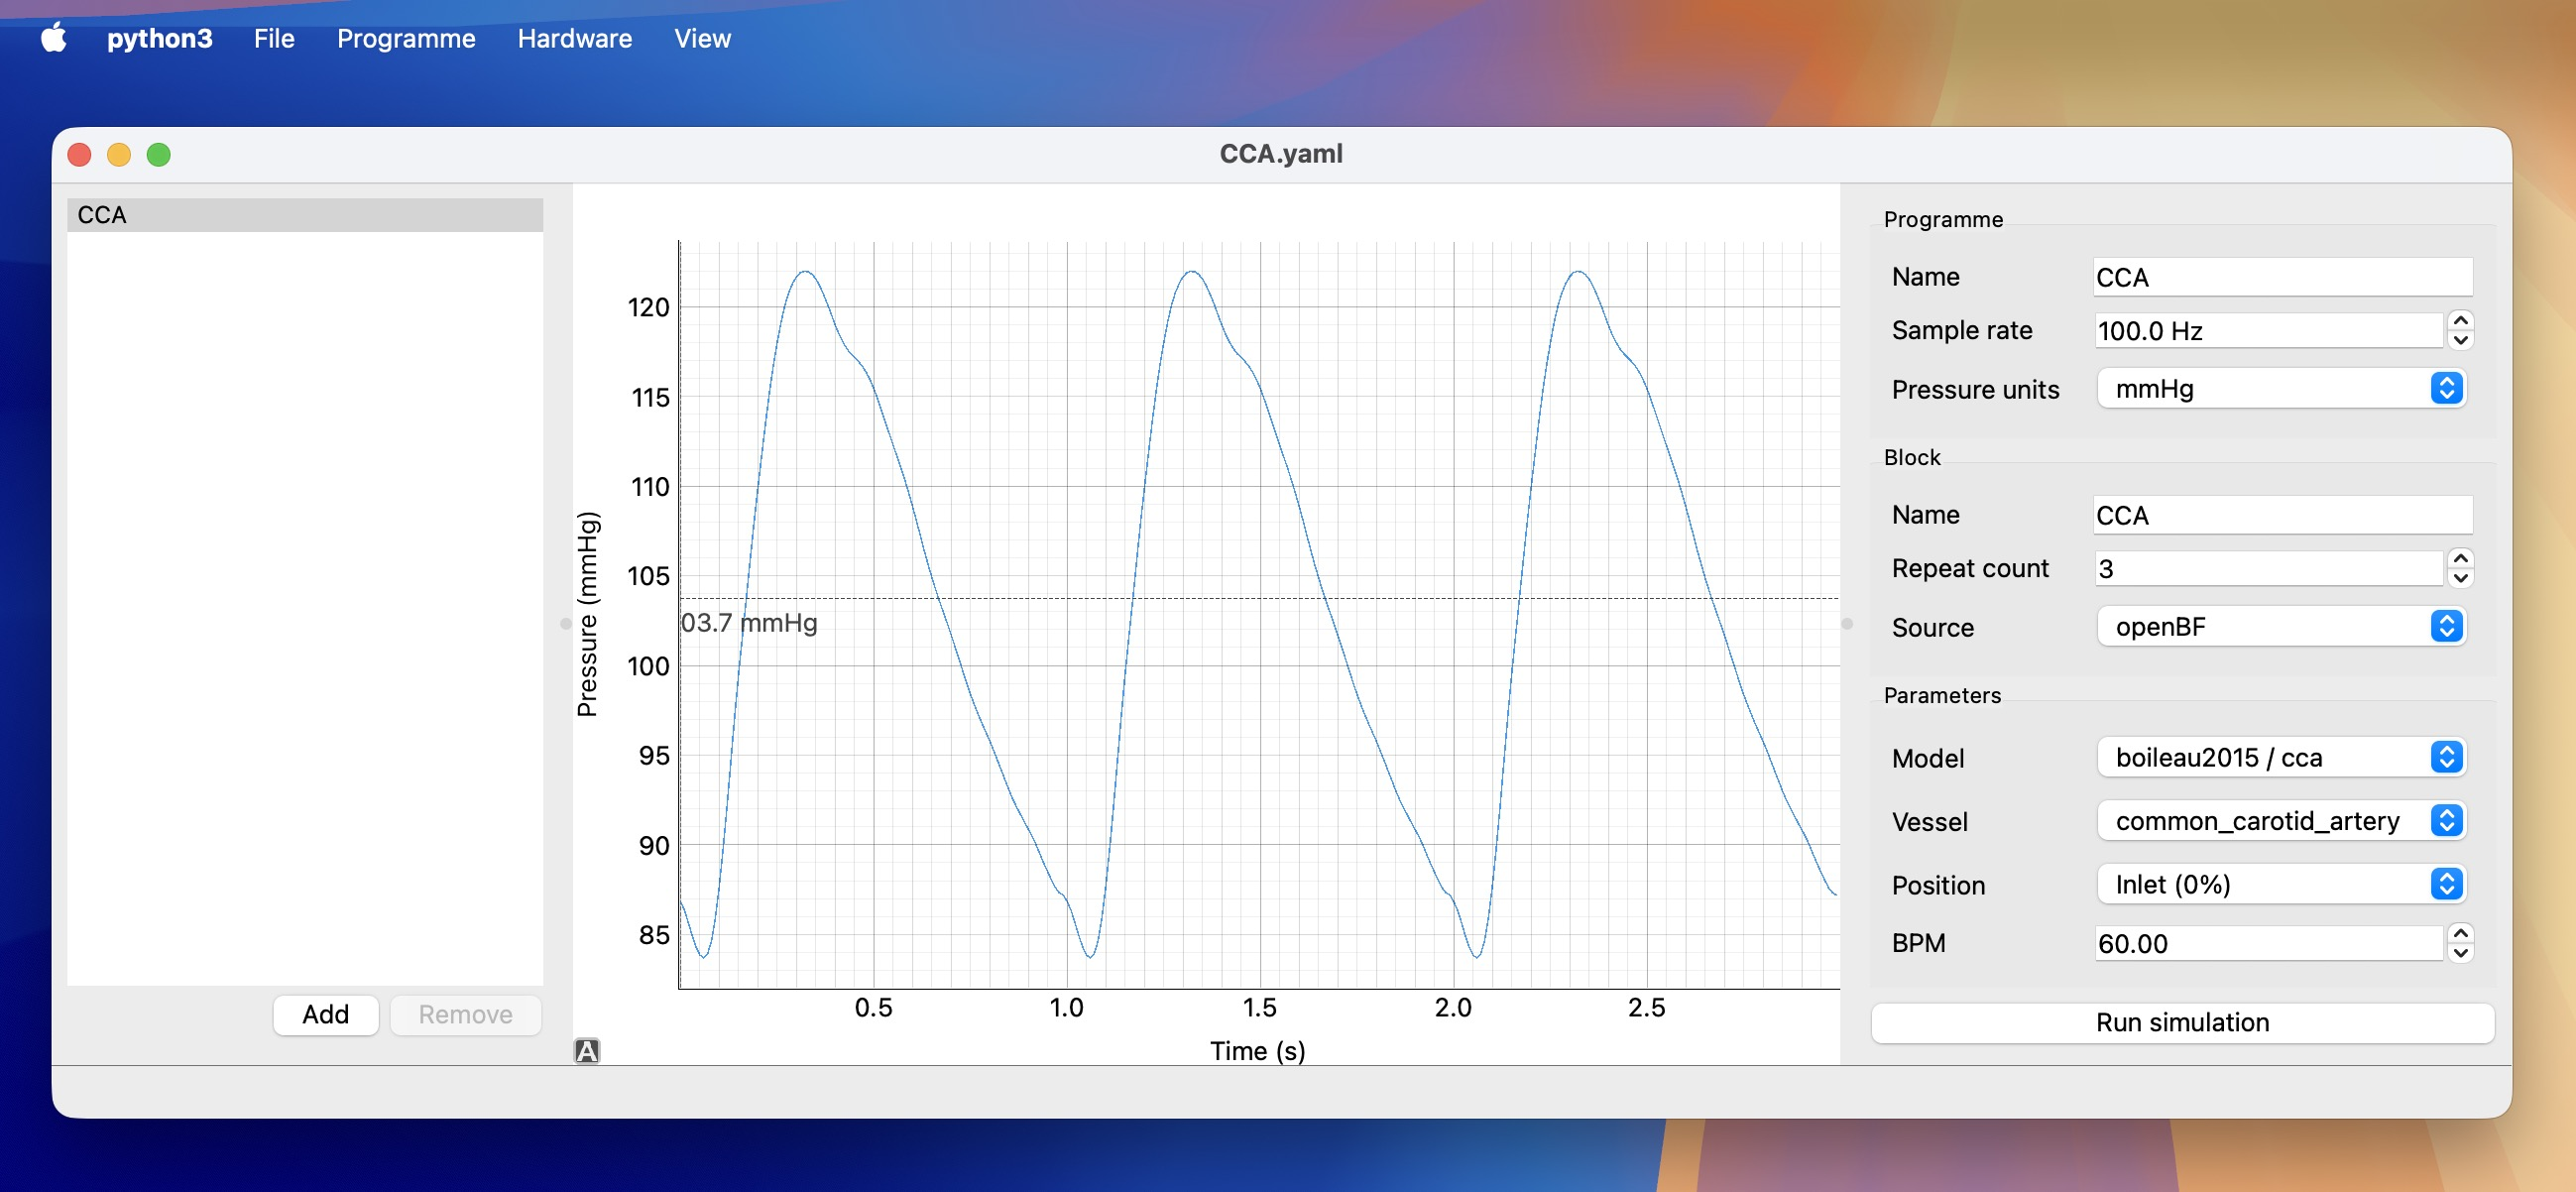
\includegraphics[width=\textwidth]{programme-editor.jpg}
  \caption{Programme editor: three-panel layout comprising a block sidebar (left), waveform preview (centre), and \Programme{}/block inspector (right).}
  \label{fig:programme-editor}
\end{figure}

\begin{figure}[H]
  \centering
  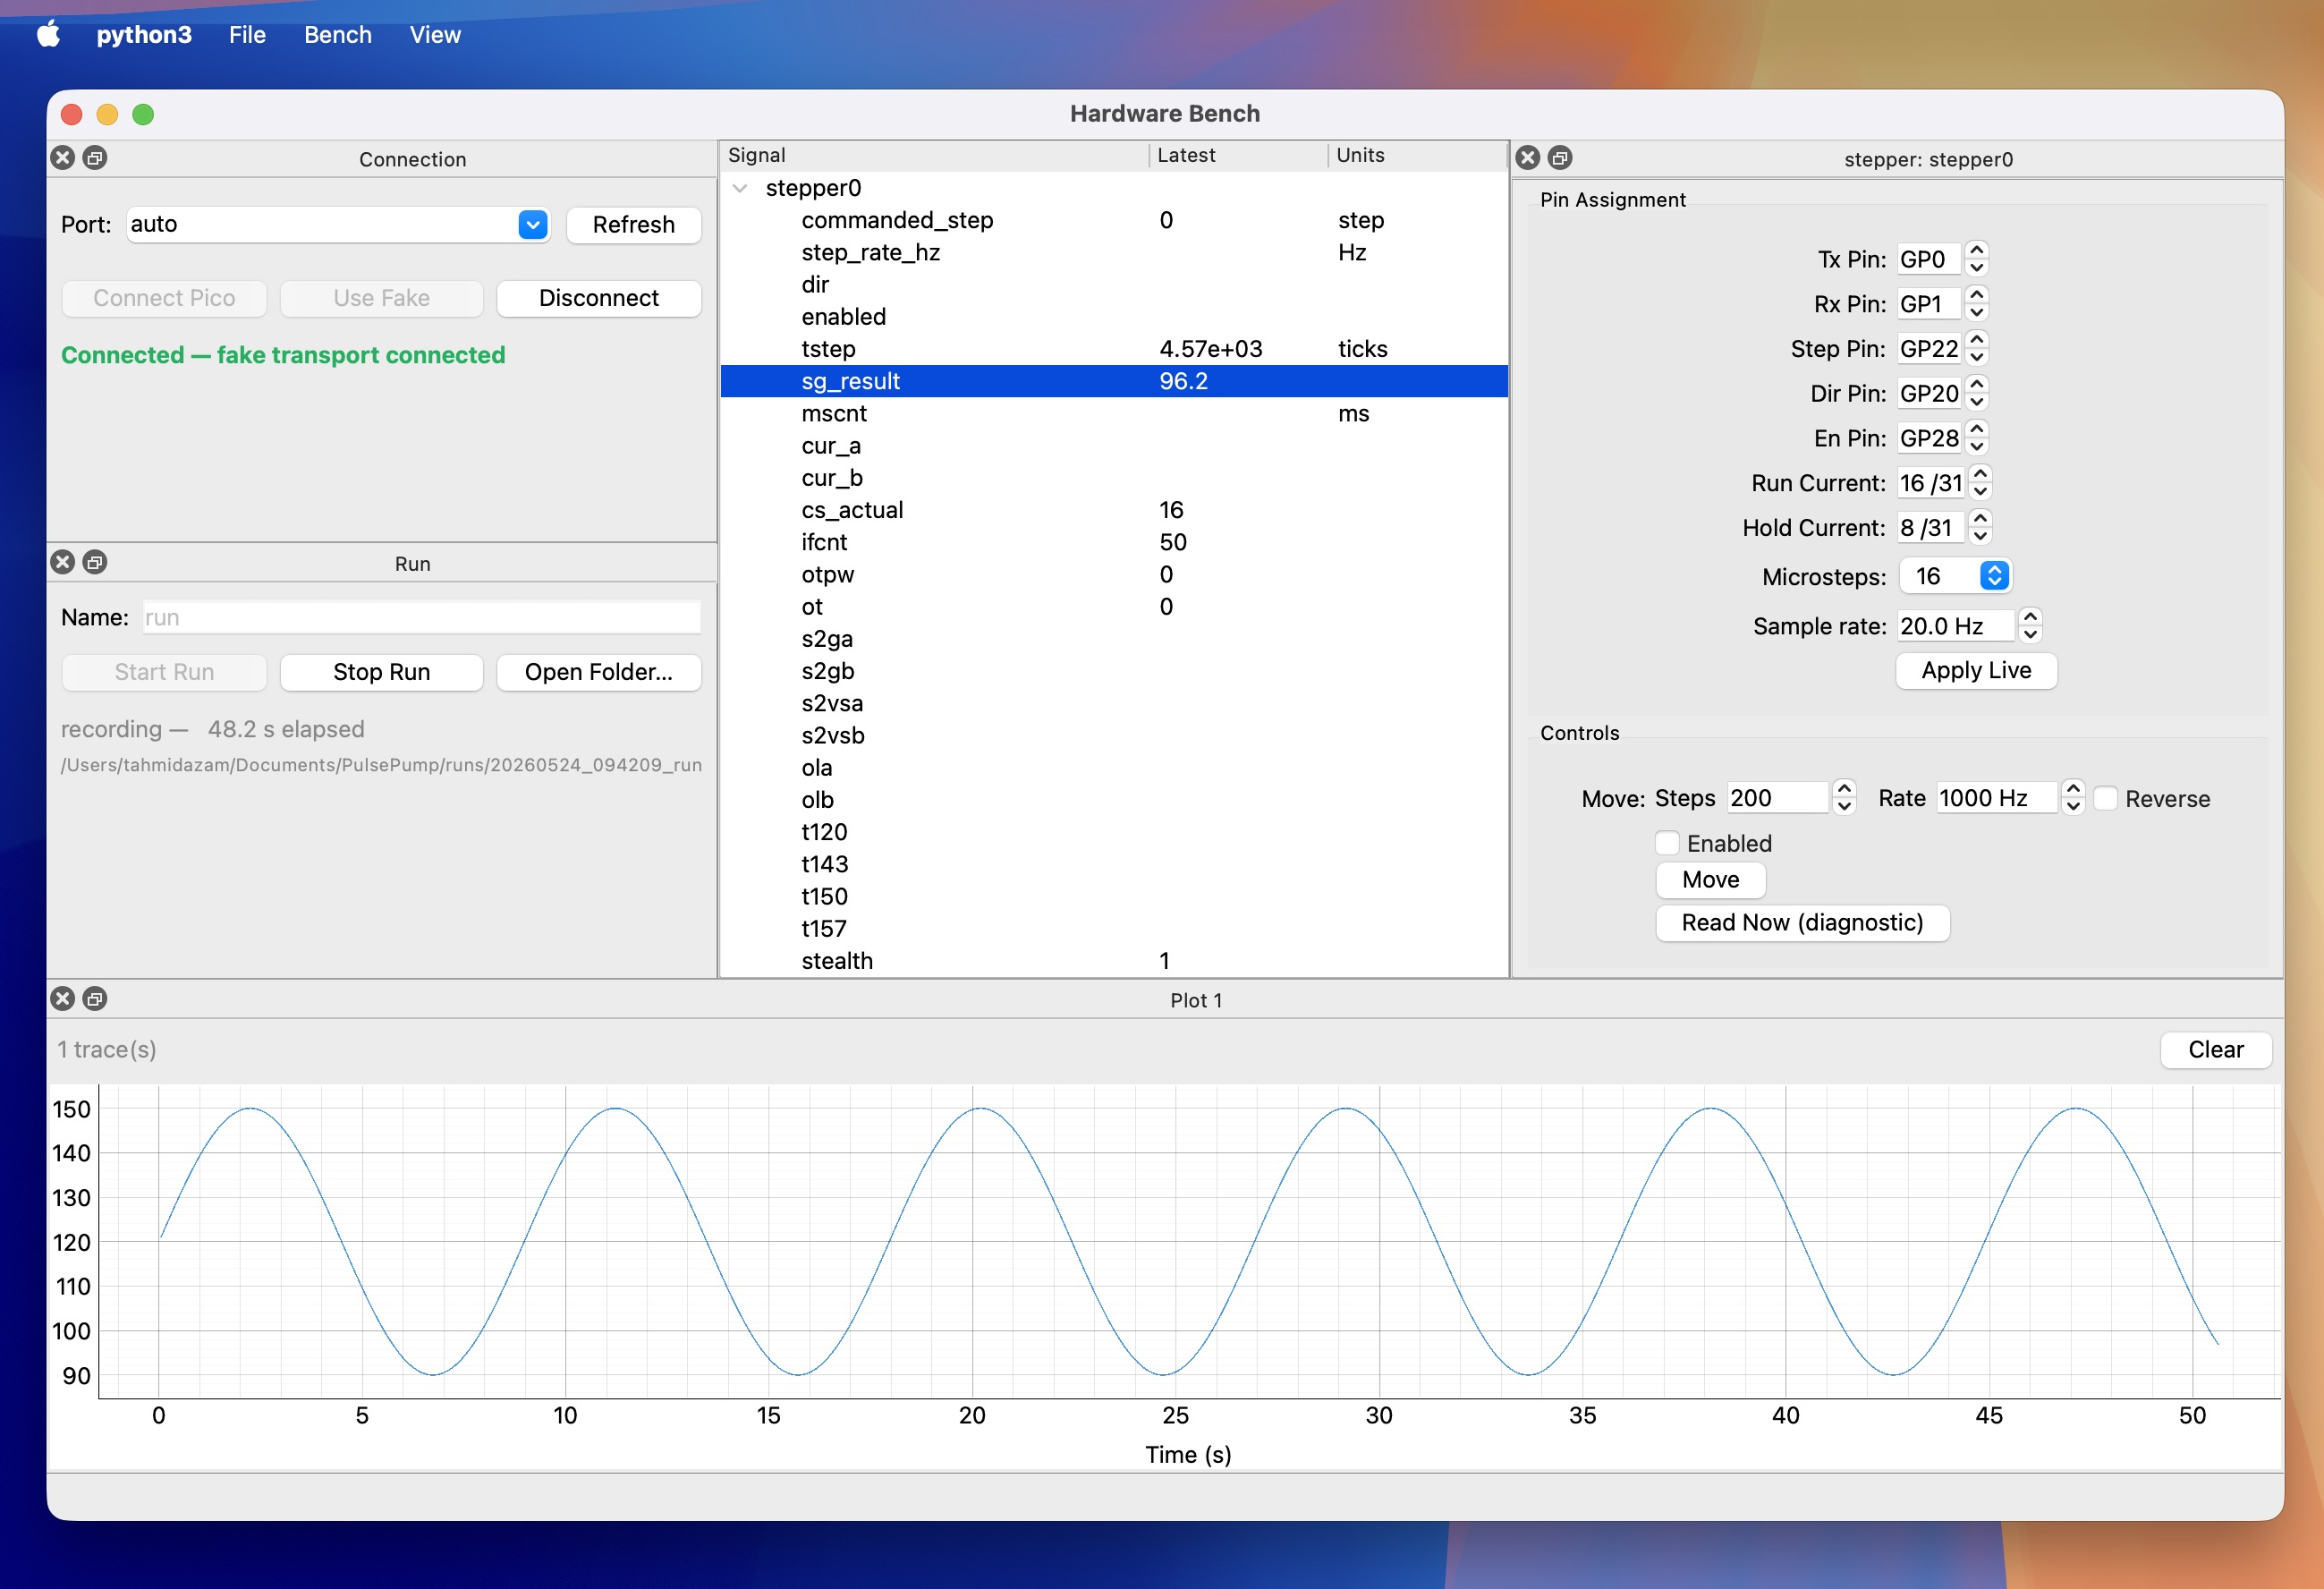
\includegraphics[width=\textwidth]{hardware-bench.jpg}
  \caption{Hardware bench: panel-based layout comprising a signals panel (centre), connection and run controls, live plot panels, and per-peripheral configuration panels. This screenshot is a mock-up using fictitious data for illustration purposes only.}
  \label{fig:hardware-bench}
\end{figure}

\end{document}
